\section{Order of Execution}
\label{sec:order-of-execution}

When discussing Audio Buses in section \ref{sec:audiobus} we hinted at the importance of order of execution. The code below is an expanded version of the filtered noise example from that section. The discussion that follows will explain the basic concept of order of execution, demonstrating why it is important.

\begin{lstlisting}[style=SuperCollider-IDE, basicstyle=\scttfamily\footnotesize]
// Create an audio bus
~fxBus = Bus.audio(s, 1);
~masterBus = Bus.audio(s, 1);
// Create SynthDefs
(
SynthDef("noise", {Out.ar(~fxBus, WhiteNoise.ar(0.5))}).add;
SynthDef("filter", {Out.ar(~masterBus, BPF.ar(in: In.ar(~fxBus), freq: MouseY.kr(1000, 5000), rq: 0.1))}).add;
SynthDef("masterOut", {arg amp = 1; Out.ar(0, In.ar(~masterBus) * Lag.kr(amp, 1))}).add;
)
// Open Node Tree window:
s.plotTree;
// Play synths (watch Node Tree)
m = Synth("masterOut");
f = Synth("filter");
n = Synth("noise");
// Master volume
m.set(\amp, 0.1);
\end{lstlisting}

First, two audio buses assigned to the variables \texttt{$\sim$fxbus} and \texttt{$\sim$masterBus}.

Second, three \texttt{SynthDef}s are created:
\begin{itemize}
\item \texttt{"noise"} is a noise source that sends white noise to an effects bus;
\item \texttt{"filter"} is a band pass filter which takes its input from the effects bus, and sends the processed sound out to the master bus;
\item \texttt{"masterOut"} takes in the signal from the master bus and applies a simple volume control to it, sending the final sound with adjusted volume to the loudspeakers.
\end{itemize}

Watch the Node Tree as you run the synths in order.

\begin{figure}[h]
\centerline{
	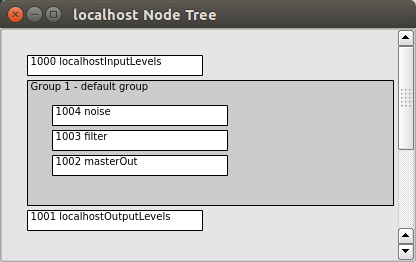
\includegraphics[scale=0.5]{fig-node-tree.png}}
\caption{Synth nodes in the Node Tree window}
\label{fig:node-tree}
\end{figure}

Synth nodes in the Node Tree window run from \emph{top to bottom}. The most recent synths get added to the top by default. In figure \ref{fig:node-tree}, you can see that \texttt{"noise"} is on top, \texttt{"filter"} comes second, and \texttt{"masterOut"} comes last. This is the right order we want: reading from top to bottom, the noise source flows into the filter, and result of the filter flows into the master bus. If you now try running the example again, but evaluating the lines \texttt{m}, \texttt{f}, and \texttt{n} in reverse order, you will hear nothing, because the signals are being calculated in the wrong order.

Evaluating the right lines in the right order is fine, but it might get tricky as your code becomes more complex. In order to make this job easier, SuperCollider allows you to explicitly define where to place synths in the Node Tree. For this we use the \texttt{target} and \texttt{addAction} arguments.

\begin{lstlisting}[style=SuperCollider-IDE, basicstyle=\scttfamily\footnotesize]
n = Synth("noise", addAction: 'addToHead');
m = Synth("masterOut", addAction: 'addToTail');
f = Synth("filter", target: n, addAction: 'addAfter');
\end{lstlisting}
Now, no matter in what order you execute the lines above, you can be sure that nodes will fall in the right places. The \texttt{"noise"} synth is explicitly told to be added to the head of the Node Tree; \texttt{"masterOut"} is added to the tail; and \texttt{filter} is explicitly added right after target \texttt{n} (the noise synth).

\subsection{Groups}

When you start to have lots of synths---some of them for source sounds, others for effects, or whatever you need---it may be a good idea to organize them into groups. Here's a basic example:

\begin{lstlisting}[style=SuperCollider-IDE, basicstyle=\scttfamily\footnotesize]
// Keep watching everything in the NodeTree
s.plotTree;

// Create some buses
~reverbBus = Bus.audio(s, 2);
~masterBus = Bus.audio(s, 2);

// Define groups
(
~sources = Group.new;
~effects = Group.new(~sources, \addAfter);
~master = Group.new(~effects, \addAfter);
)

// Run all synths at once
(
// One source sound
{
  Out.ar(~reverbBus, SinOsc.ar([800, 890])*LFPulse.ar(2)*0.1)
}.play(target: ~sources);

// Another source sound
{
  Out.ar(~reverbBus, WhiteNoise.ar(LFPulse.ar(2, 1/2, width: 0.05)*0.1))
}.play(target: ~sources);

// Some reverb
{
  Out.ar(~masterBus, FreeVerb.ar(In.ar(~reverbBus, 2), mix: 0.5, room: 0.9))
}.play(target: ~effects);

// Some silly master volume control with mouse
{
  Out.ar(0, In.ar(~masterBus, 2) * MouseY.kr(0, 1))
}.play(target: ~master);
)
\end{lstlisting}

For more information about order of execution, look up the Help files ``Synth,'' ``Order of Execution,'' and ``Group.''